\documentclass[12pt]{article}
 
\usepackage[margin=1in]{geometry} 
\usepackage{amsmath,amsthm,amssymb,graphicx,mathtools,tikz,hyperref}
\usepackage{indentfirst}
\usepackage{ragged2e}
\RaggedRightParindent = 24 pt
\setlength{\parskip}{1.5em}
\usepackage{algorithm2e}
\usepackage{graphicx}
\usepackage{titling}
\renewcommand\maketitlehooka{\null\mbox{}\vfill}
\renewcommand\maketitlehookd{\vfill\null}
\usepackage{tocloft}
\renewcommand\cftsecafterpnum{\vskip6pt}

\usepackage{mdframed}

\newenvironment{res}
    { \begin{mdframed}[backgroundcolor=orange!10]}
    {  \end{mdframed}}
    
\usepackage{xcolor}
\usepackage{listings}
\lstset{basicstyle=\ttfamily,
  showstringspaces=false,
  commentstyle=\color{red},
  keywordstyle=\color{blue}
}
 
\definecolor{commentext}{RGB}{0, 0, 102}
\definecolor{score}{RGB}{153, 0, 0}


\definecolor{bluekeywords}{rgb}{0.13,0.13,1}
\definecolor{greencomments}{rgb}{0,0.5,0}
\definecolor{turqusnumbers}{rgb}{0.17,0.57,0.69}
\definecolor{redstrings}{rgb}{0.5,0,0}

\lstdefinelanguage{bash}
    {morekeywords={let,insertOne,insertMany, update, replace, updateOne, updateMany, toArray,gt,lt,lte,gte, findOne,find,deleteOne, deleteMany,db, show, use, mongod, mongo, import, as, public, class, void, static, echo, new, match, with, rec, open, module, namespace, type, of, member, and, for, in, do, begin, end, fun, function, try, mutable, if, then, else},
    keywordstyle=\color{bluekeywords},
    sensitive=false,
    morecomment=[l][\color{greencomments}]{///},
    morecomment=[l][\color{greencomments}]{//},
    morecomment=[s][\color{greencomments}]{{(*}{*)}},
    morestring=[b]",
    stringstyle=\color{redstrings}
    }

\lstnewenvironment{code}
  {
    \lstset{
        language=bash,
        basicstyle=\ttfamily,
        breaklines=true,
        columns=fullflexible,
        backgroundcolor = \color{orange!10}}
  }
  {
  }


\begin{document}
\title{Practical Understanding of DFT}
\author{Sizhe Liu\\Department of Mechanical Science and Engineering \\University of Illinois at Urbana-Champaign\\ } 
\date{Version 3.14}
\begin{titlingpage}
\maketitle
\end{titlingpage}

\newpage
\tableofcontents
\newpage
\vspace*{100pt}
\textit{We must know, especially when it is effortless to know.}
\newpage

\section{Some Basic Definitions/Approx.}
\textbf{\textit{Ground state}}: the lowest energy state of the electrons.

\textbf{\textit{Born-Oppenheimer approximation}} (BOA): the separation of the nuclei and electrons into two mathematical problems.

\textbf{\textit{Adiabatic potential energy surface}}: The ground-state energy function taking the positions of nuclei as arguments.

\textbf{\textit{Time-independent nonrelativistic Schrodinger Equation}}:

\begin{equation}
    [-\frac{\hbar^2}{2m}\sum^N_{i=1}\nabla^2_i+\sum^N_{i=1}V(\boldsymbol{r}_i)+\sum_{i=1}^N\sum_{j<i}U(\boldsymbol{r}_i, \boldsymbol{r}_j)]\psi = E\psi
\end{equation}
where $V(\boldsymbol{r}_i)$ is the energy arises from interactions among electrons, and $U(\boldsymbol{r}_i, \boldsymbol{r}_j)$ is the potential energy for nuclei-electron interactions. The N-electron wavefunction $\psi$ can be approximate by a Hartree product:$\psi=\psi_1(\boldsymbol{r})\psi_2(\boldsymbol{r})...\psi_N(\boldsymbol{r})$.

\textbf{\textit{Density of electrons}} at a particular position in space:  $n(\boldsymbol{r})=2\sum_i\psi^*_i(\boldsymbol{r})\psi_i(\boldsymbol{r})$.Here, the factor of \textit{2} appears because electrons have \textit{spin and the Pauli exclusion principle states that each individual electron wave function can be occupied by two separate electrons provided they have different spins.}

\textbf{\textit{Functional}}: A functional takes a function and defines a single number from the function, a mapping from one function to another function. Integral such as:
\begin{equation}
    f \mapsto I[f]=\int_\Omega \mathcal{H}(f(x),f`(x),...) d^nx
\end{equation}
forms a special class of functional widely used in DFT.

\textbf{\textit{Reciprocal Space}}: The space of vectors \emph{r} is called real space, and the space of wave vectors \emph{k} is called reciprocal space.

\textbf{\textit{Brillouin Zone}}: The primitive lattice cell defined in reciprocal space.

\textbf{\textit{Hohenberg-Kohn first theorem}}: \emph{The ground-state energy from Schrodinger's equation is a unique fuctional of the electron density}. Hohenberg and Kohn proved that there exists a one-to-one mapping between the ground-state wave function and the \textit{ground state electron density}:\textbf{$E=E[n(\boldsymbol{r})]$}.

\textbf{\textit{Hohenberg-Kohn second theorem}}:\textit{The electron density that minimizes the energy of the overall functional is the true electron density corresponding to the full solution of the Schrodinger equation.}

\textbf{\textit{Hohenberg-Kohn functional}}: One way to write down the functional in terms of the \textit{single-electron} wave functions:
\begin{equation}
    E[{\psi_i}]=E_{known}[{\psi_i}]+E_{XC}[{\psi_i}]
\end{equation}
where we have simple analytical energy $E_{known}$ and quantum-mechanical energy functional (i.e., exchange-correlation functional) $E_{XC}$. The analytical energy includes four contributions: the electron kinetic energies, the electron-nuclei Coulomb interactions, the electron-electron Coulomb interactions, and the nuclei-nuclei Coulomb interactions, as shown in the equation below:
\begin{equation}
    E_{known}[{\psi_i}]=-\frac{\hbar^2}{m}\sum_i\int\psi^*_i\nabla^2\psi_idr+\int V(\boldsymbol{r})n(\boldsymbol{r})dr+e^2/2\iint\frac{n(\boldsymbol{r})n(r')}{|r-r'|}drdr' + E_{nuclei-nuclei}
\end{equation}

\textbf{\textit{Kohn-Sham equations}}: The difficulty of finding the electron density can be solved by solving a set of single-electron equations. These equations have the form:
\begin{equation}
    [-\frac{\hbar^2}{2m}\nabla^2+V(\boldsymbol{r})+V_H(\boldsymbol{r})+V_{XC}(\boldsymbol{r})]\psi_i(\boldsymbol{r})=\epsilon_i\psi_i(\boldsymbol{r})
\end{equation}
where $V(\boldsymbol{r})$ defines the interaction between an electron and the collection of atomic nuclei. The Hartree potential $V_H(\boldsymbol{r})=e^2\int\frac{n(r')}{|r-r'|}dr'$ describes the Coulomb repulsion between the electron being considered in one of the Kohn-Sham equations and the total electron density defined by all electrons in the problem. \textit{Because the electron described in the Kohn-Sham equation is also part of the total electron density,} \textbf{so part of $V_H$ involves a Coulomb interaction between the electron and itself.}(i.e., \emph{self-interaction}). The correction for the self-interaction is integrated into $V_{XC}$.

\textbf{\textit{Self-consistency algorithm}}: A pseudo-code to solve electron density is shown here.
\begin{algorithm}
\SetAlgoLined
\KwResult{Electron density $n(\boldsymbol{r})$ }
 initialize $n_0(\boldsymbol{r})$, $n_{new}(\boldsymbol{r})$, and threshold $\epsilon$\;
 \While{$|n_0-n_{new}|>\epsilon$}{
  $n_0 = n_{new}$\;
  Solve $Kohn-Sham$ equation to get $\psi_i(\boldsymbol{r})$\;
  Calculate $n_{new}(\boldsymbol{r})=2\sum_i\psi^*(\boldsymbol{r})\psi(\boldsymbol{r})$
  
 }
 $n(\boldsymbol{r})=n_{new}(\boldsymbol{r})$
\caption{Calculate Electron Density}
\end{algorithm}

\textbf{\textit{Local density approximation (LDA)}}: The $V_{XC}$ at each position is set to be the known exchange-correlation potential from the uniform electron gas observed at that position.(i.e., $V_{XC}=V_{XC}^{\textit{electron gas}}[n(\boldsymbol{r})]$).

\textbf{\textit{Generalized gradient approximation (GGA)}}: $V_{XC}=V_{XC}^{\textit{electron gas}}[n(\boldsymbol{r}), \nabla n(\boldsymbol{r})]$.

\textbf{\textit{Wave-Function-Based Methods}}: Unlike DFT, which solves for electron density, wave-function-based methods aim at calculating full electron wave function.

\textbf{\textit{Miller index of lattice surface}}: specify the points at which the plane intersects the three axes of the material's primitve cell or the conventional cell. The reciprocals of these intercepts are then multiplied by a scaling factor that makes each reciprocal an integer and also makes each integer as small as possible. The resulting set of numbers is called the \emph{Miller index} of the surface.

\textbf{\textit{Minimum energy path}}(MEP): the process path connecting two local minima of the energy landscape through saddle points.

\textbf{\textit{Crossover temperature}}: A critical temperature to evaluate the contribution of quantum tunneling to the total chemical process rate. Below the crossover temperature, tunneling can make a significant contribution to the total rate, while above this temperature tunneling can be neglected.

\section{Side Notes on Hartree-Fock Method and Beyond}
Hartree-Fock method is a wave-function-based method, which solves single-electron equation, and uses Slater determinant to construct full wave function for many-electron systems.

Suppose we would like to approximate the wave function of N electrons. Let us first assume that the electrons have \textit{no effect} on each other. Then, the Hamiltonian for the electrons may be written as:
\begin{equation}
    \mathcal{H} = \sum_{i=1}^N h_i
\end{equation}
where $h_i$ describes the kenetic and potential energy of electron "\textit{i}". Then, the Schrodinger equation for just one electron is:
\begin{equation}
    h\chi = E\chi
\end{equation}
where the eigenfunctions $\chi$ defined here are called \textit{spin orbitals}. For each single-electron equation there are multiple eigenfunctions, so this defines a set of spin orbitals $\chi_j(\boldsymbol{x}_i)(j=1,2,...)$ where $\boldsymbol{x}_i$ is a vector of coordinates defining the coordinates and the spin state of electron \textit{i}. When the total Hamiltonian is simply a sum of one-electron operators, it follows that the eigenfunctions of $\mathcal{H}$ are products of the one-electron spin orbitals (i.e., Hartree product). Unfortunately, the construction of Hartree product does not satisfy the antisymmetry principle as the product's sign does not change if two electrons exchange their places. Thus, we use a Slater determinant as a better approximation to the wave function. For two electrons, the Slater determinant is:
\begin{equation}
    \psi(\boldsymbol{x}_1, \boldsymbol{x}_2) = \frac{1}{\sqrt{2}}det
  \left[ {\begin{array}{cc}
   \chi_j(\boldsymbol{x}_1) & \chi_j(\boldsymbol{x}_2)\\
   \chi_k(\boldsymbol{x}_2) & \chi_k(\boldsymbol{x}_1) \\
  \end{array} } \right]
\end{equation}

The Slater determinant satisfies the conditions of the Pauli exclusion principle as it disappears if two electrons have the same coordinates or if two of the one-electron wave functions are the same. For a system of N electrons, the Slater determinant is the determinant of an $N\times N$ matrix of spin orbitals. Unfortunately, the Slater determinant along is \emph{not enough to include all kinds of electron correlations}.

In a Hartree-Fock (HF) calculation, the Schrodinger equation is solved for each electron. The equation is written as:
\begin{equation}
    \label{HFeq}
    [-\frac{\hbar^2}{2m}\nabla^2+V(\boldsymbol{r})+V_H(\boldsymbol{r})]\chi_j(\boldsymbol{x}) = E_j\chi_j(\boldsymbol{x})
\end{equation}
where $V_H(\boldsymbol{r})$ is the same Hartree potential used in the \textit{Kohn-Sham equations}. Unlike DFT, $V_H$ in HF describes how each electron "\textit{feels}" the effect of other electrons \textbf{\emph{only as an average}}. rather than feeling the \emph{instantaneous repulsive forces generated as electrons become close in space}. The $V_{XC}$ does not appear in the equation above because the Slater determinant captures the exact form of the electron exchange effect.

To actually solve the equation \ref{HFeq}, HF method defines a finite set of basis functions $\phi_i$ to approximate the spin orbitals:
\begin{equation}
    \chi_j(\boldsymbol{x}) = \sum_{i=1}^K\alpha_{j,i}\phi_i(\boldsymbol{x})
\end{equation}
The spatially localized functions can be used as $\phi_i$ for the calculation of isolated molecules while periodically fluctuated functions are usually chosen for the bulk material calculations. 

We now have all the pieces in place to perform an HF calculation. Like DFT, an HF calculation is also an iterative procedure that can be outlined as follows:

\begin{algorithm}[H]
\SetAlgoLined
\KwResult{Full wave function $\psi$ }
 initialize $\chi_j(\boldsymbol{x}),\chi'_j(\boldsymbol{x})$ by specifying the expansion coefficient $\alpha_{j,i}$ and $\epsilon$\;
 \While{$|\chi_j(\boldsymbol{x})-\chi'_j(\boldsymbol{x})|>\epsilon$}{
  $\chi_j(\boldsymbol{x})=\chi'_j(\boldsymbol{x})$\;
  Define the electron density $n(\boldsymbol{r})$ from the Slater determinant\;
  Solve the equation \ref{HFeq} for $\chi'_j(\boldsymbol{x})$ using $n(\boldsymbol{r})$ from the previous step\;
  Calculate $n_{new}(\boldsymbol{r})=2\sum_i\psi^*(\boldsymbol{r})\psi(\boldsymbol{r})$
 }
 $\chi_j(\boldsymbol{x})=\chi'_j(\boldsymbol{x})$
 
 $\psi(\boldsymbol{x}_1,\boldsymbol{x}_2,...,\boldsymbol{x}_N)=\frac{1}{\sqrt{N!}}det[\chi_j(\boldsymbol{x}_i)]$
\caption{HF Calculation}
\end{algorithm}
\subsection{Beyond Hartree-Fock}
If HF calculations were possibly using an infinitely large set of basis functions, the energy of N electrons that would be calculated is known as the "\textit{Hartree-Fock limit}". This energy is not the same as the energy for the true electron wave function because the HF method does not correctly describe how electrons influence other electrons. More succinctly, the HF method \textbf{does not deal with electron correlations}.

Writing down the physical laws that govern electron correlation is straightforward, but finding an exact description of electron correlation is in tractable for any but the simplest system. Therefore, the electron correlation is defined, within the context of quantum chemistry, as \textbf{the difference between the Hartree-Fock limit and the true non-relativistic ground-state energy}.

The common goal of constructing a more advanced approach upon HF method is to include a description of electron correlation. Electron correlation is often described by "mixing" into the wave function some configurations in which electrons have been excited to higher energy orbitals. Several groups of methods that do this are listed below:

\textbf{\emph{Single-determinant methods}}: A single Slater determinant is used as the reference wave function and excitations are made from the reference. These methods include configuration interaction (\textbf{CI}), coupled cluster (\textbf{CC}), Moller-Plesset perturbation theory (\textbf{MP}), and the quadratic configuration interaction (\textbf{QCI}) approach. Ech of these methods has multiple variants. For example \textbf{CCSD} is coupled-cluster calculations involving excitations of single electrons (S), and pairs of electrons (D), while \textbf{CCSDT} includes excitations of three electrons (T). On the other hand, \textbf{MP2} is a second-order perturbation theory.

\textbf{\emph{Multiple-determinant methods}}: these methods use multiple Slater determinants as the reference. The description of electron correlation within these methods are somewhat similar to the methods listed above. These methods include multiconfigurational self-consistent field (\textbf{MCSCF}), multireference single and double configuration interaction (\textbf{MRDCI}).

\emph{The longer the acronym, the better the level of theory.}

\subsubsection{Electron correlation in DFT}
The electron correlation is described by \emph{exchange-correlation} functional (i.e.,$V_{XC}$) in DFT. The most commonly used functionals in DFT based on spatially localized basis functions are "\textbf{hybrid}" functionals (e.g., B3LYP). These functionals \textit{mix the \textbf{exact exchange part} of the functionals with approximations for the correlation part}.

Unfortunately, the form of the exact exchange results mean that the "hybrid" functionals can be efficiently implemented for applications based on spatially localized functions but \textit{not for applications using periodic functions}. Because of this, the functionals that are commonly used in plane-wave DFT calculations do not include contributions from the \emph{exact exchange results}.

\section{Phase Transformations Analysis with DFT}
For crystal materials, the structure with the lowest energy is preferred by nature. To make this argument more precise, we need to carefully define a material's energy as the Gibbs free energy, $G=G(P, T)$. The Gibbs free energy can be written as:
\begin{equation}
    G(P, T) = E_{coh} + PV - TS
\end{equation}
where $E_{coh}$, V, and S are the cohesive energy (i.e., the energy to pull a material apart into a collection of isolated atoms), volume, and entropy of a material. If we are comparing two possible crystal structures, then we are interested in the Gibbs free energy difference:
\begin{equation}
    \Delta G(P,T)=\Delta E_{coh}+P\Delta V - T \Delta S
\end{equation}
The change in cohesive energy between the two structures is just the difference between the DFT total energies.In solides, the first two terms tend to be \emph{much larger than }the entropic contribution, so
\begin{equation}
    \label{gibbs}
    \Delta G(P,T)\cong\Delta E_{coh}+P\Delta V 
\end{equation}
\begin{equation}
    P=-\frac{\partial E_{coh}}{\partial V} 
\end{equation}

An interesting consequence of equation\ref{gibbs} is that \emph{teo crystal structures with different cohesive energies can have the same Gibbs free energy if }$\Delta E_{coh}=-P\Delta V$. Now, we can see that two structures satisfy this condition if they share a \textbf{common tangent }on a plot of $\Delta E_{coh}$ as a function of $V$.
\begin{figure}[h]
\caption{Schematic illustration of a pressure-induced transformation between two crystal
structures of a material}
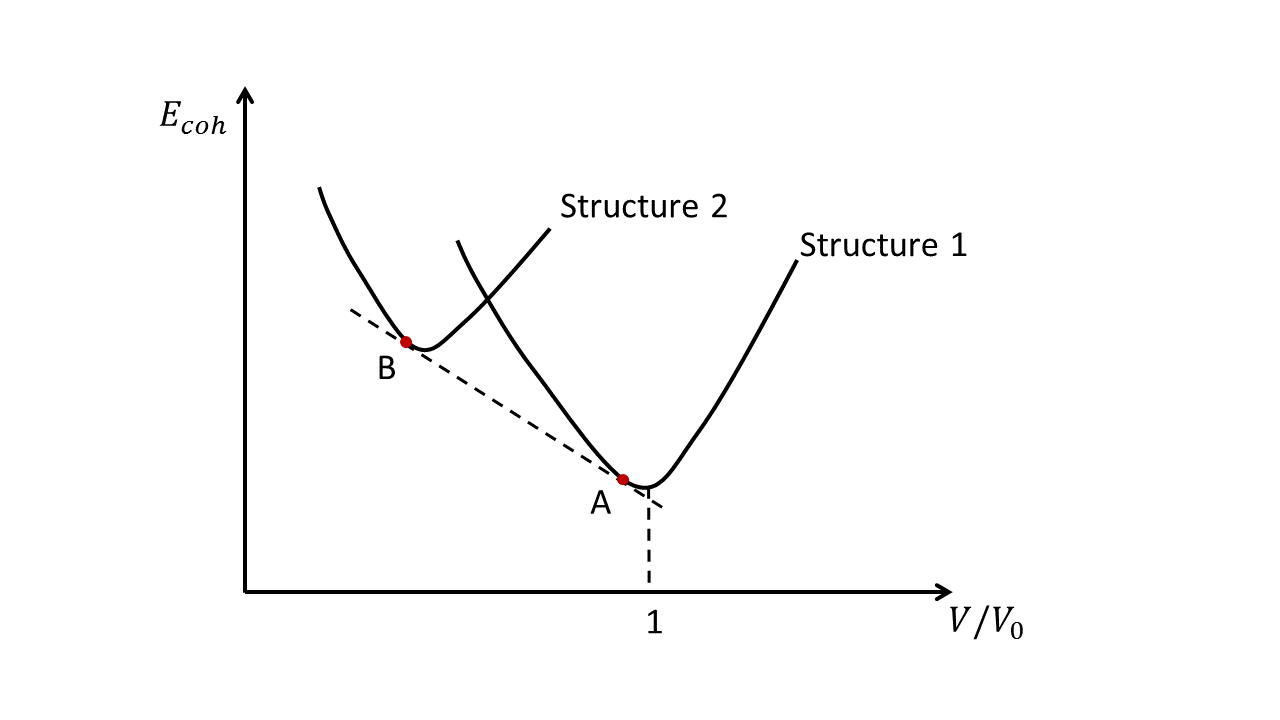
\includegraphics[width=\textwidth]{pic01.png}
\end{figure}

In the figure 1, the preferred crystal structure at P = 0 is structure 1, and the lattice parameter of this preferred structure defines a volume V0. Moving along the curve for the cohesive energy from the minimum at V/V0 = 1 toward the point labeled A is equivalent to increasing the pressure on the material. When the pressure corresponding to point A is reached, the curve for structure 1 shares a common tangent with structure 2. At higher pressures, the Gibbs free energy of structure 2 is lower than for structure 1, so the figure predicts that a pressure induced phase transformation would occur at this pressure that would change the crystal structure of the material. In this phase change the cohesive energy goes up, but this change is balanced within the free energy by the reduction in the volume of the material.

\section{The ideas behind \textit{k} Points}
If we solve the Schrodinger equation for periodic systems, the solution must satisfy a fundamental property known as \textbf{Bloch's theorem}, which states that the solution can be expressed as a sum of terms with the form
\begin{equation}
    \phi_k(\boldsymbol{r})=exp(i\boldsymbol{k}\cdot\boldsymbol{r})u_k(\boldsymbol{r}),
\end{equation}
where $u_k(\boldsymbol{r})$ is periodic in space with the same periodicity as the supercell. This theorem means that \textbf{it is possible to try and solve the Schrodinger equation for each value of $\boldsymbol{k}$ independently}.It turns out that many parts of the mathematical problems posed by DFT are much more convenient to solve in terms of $\boldsymbol{k}$ than they are to solve in terms of r. Because the functions
$exp(i\boldsymbol{k}\cdot\boldsymbol{r})$ are called \textit{plane waves}, calculations based on this idea are frequently referred to as \textit{plane-wave calculations}.

The idea of Brillouin zone and \emph{k} points are important because in a practical DFT calculation, a great deal of the work reduces to evaluating integrals of the form:
\begin{equation}
    \bar g = \frac{V_{cell}}{(2\pi)^3}\int_{BZ}g(\boldsymbol{k})d\boldsymbol{k}
\end{equation}
Since integrals can be approximated by evaluating the function to be integrated at a set of discrete points and summing the function values with appropriate weighting for each point, we need to carefully choose \emph{k points}.

\textbf{The key ideas related to getting well-converged results in k space include:}

1. Before pursuing a large series of DFT calculations for a system of interest, numerical data exploring the convergence of the calculations with respect to the number of k points should be obtained.

2. The number of k points used in any calculation should be reported since not doing so makes reproduction of the result difficult.

3. Increasing the volume of a supercell reduces the number of k points needed to achieve convergence because volume increases in real space correspond to volume decreases in reciprocal space.

4. If calculations involving supercells with different volumes are to be compared, choosing k points so that the density of k points in reciprocal space is comparable for the different supercells is a useful way to have comparable levels of convergence in k space.

\section{Notes on Cutoff Energy, Pseudopotential, and Geometry Optimization}
\subsection{Cutoff energy}
According to Bloch's theorem, the solutions of the Schrodinger equation for a supercell have the form:
\begin{equation}
    \phi_{\boldsymbol{k}}(\boldsymbol{r})=exp(i\boldsymbol{k\cdot r})u_{\boldsymbol{k}}(\boldsymbol{r})
\end{equation}
where $u_{\boldsymbol{k}}(\boldsymbol{r})$ is periodic in space with the same periodicity as the supercell. The periodicity of  $u_{\boldsymbol{k}}(\boldsymbol{r})$ means that it can be expanded in terms of a special set of plane waves:
\begin{equation}
    u_{\boldsymbol{k}}(\boldsymbol{r})=\sum_{\boldsymbol{G}}C_{\boldsymbol{G}}exp[i\boldsymbol{G}\cdot \boldsymbol{r}]
\end{equation}
where the summation is over all vectors defined by $G=m_1b_1+m_2b_2+m_3b_3$ with integer values for $m_i$. These set of vectors defined by $\boldsymbol{G}$ in reciprocal space are defined so that for any real space lattice vector $\boldsymbol{a}_i$, $\boldsymbol{G}\cdot \boldsymbol{a}_i=2\pi m_i$. Combining the information above gives:
\begin{equation}
    \phi_{\boldsymbol{k}}(\boldsymbol{r})=\sum_{\boldsymbol{G}}C_{\boldsymbol{k+G}}exp(i\boldsymbol{(k+G)\cdot r})
\end{equation}
The function above has a simple interpretation as solutions of the Schrodinger equation: they are solution with kinetic energy
\begin{equation}
    E = \frac{\hbar^2}{2m}|\boldsymbol{k}+\boldsymbol{G}|^2
\end{equation}

It is reasonable to expect that the solutions with lower energies are more physically important than solutions with very high energies. As a result, it is usual to truncate the infinite sum above to include only solutions with kinetic energies less than some value:
\begin{equation}
    E_{cut}=\frac{\hbar^2}{2m}G^2_{cut}
\end{equation}
The infinite sum then reduces to 
\begin{equation}
    \phi_{\boldsymbol{k}}(\boldsymbol{r})=\sum_{\boldsymbol{|G+k|}<G_{cut}}C_{\boldsymbol{k+G}}exp(i\boldsymbol{(k+G)\cdot r})
\end{equation}
This expression includes slightly different numbers of terms for different values of $\boldsymbol{k}$.

The discussion above introduces one more parameter that must be defined in DFT calculation--the cutoff energy $E_{cut}$.
\subsection{Pseudopotentials}
It is natural to think that large energy cutoffs must be adopted to include plane waves that oscillate on short length scales in real space. This is problematic because \textbf{the tightly bound core electrons} in atoms are associated with wave functions with exactly this kind of oscillation.Thus, high-frequency plane wave functions could cause numerical divergence in the calculation of core electrons. From a physical point of view, however, core electrons are not especially important in defining chemical bonding and other physical characteristics of materials. So it was clear that there could be great advantages in calculations to reduce the computational burden due to core electrons. Conceptually, a pseudopotential replaces the electron density from a chosen set of core electrons with a smoothed density chosen to match various important physical and mathematical properties of the tron \textit{ion core}. The properties of the core electrons are then \emph{fixed in this approximate fashion in all subsequent calculations; this is the \textbf{frozen core approximation}}.

A pseudopotential requiring high cutoff energies are said to be hard, while more computationally efficient pseudopotentials with low cutoff energies are soft. The most widely used pseudopotentials are the ultrasoft pseudopotentials (USPPs). One disadvantage of using USPPs is that the construction of the pseudopotential for each atom requires a number of empirical parameter to be specified. Current DFT codes typically only include USPPs that have been carefully developed and tested, but they do in some cases include USPPs with varying degrees of softness for some elements. Another frozen core approach that avoids some of the disadvantages of USPPs is the \textit{projector augmented-wave}(\textbf{PAW}) method. \textbf{In materials with strong magnetic moments or with atoms that have large differences in electronegativity, the PAW approach gives more reliable results than USPPSs.}

\subsection{Geometry optimization}
In a structural relaxation calculation, we usually setup a convergence threshold value for atomic force as a criterion to stop calculation. A typical value for force criterion is $0.01 eV/Angstrom$. Why is this force criterion reasonable? If we change an atom's position by a small amount, $\Delta r$, then the change in total energy due to the change can be estimated by $|\Delta E|=|\boldsymbol{F}\cdot \Delta r|$, where $\boldsymbol{F}$ is the force on the atom. If the forces on all atoms are less than $0.01 eV/Angstrom$, then moving any individual atom by $0.1$ Angstrom, a relatively significant distance in terms of chemical bonding, will change the total energy by less than 0.001 eV, a small amount of energy.

\section{DFT for Solid Surface Modeling}
If our goal is to study a surface, our model should be a slice of material that is infinite in teo dimensions, but finite aling the surface normal. To accomplish this, we can take advantage of periodic boundary condition in all three dimensions. In the supercell box, the atoms at the lower portion of the box fill the entire space in the $x$ and $y$ directions, but empty space has been left above the atoms in the top portion of the supercell. This model is called a \textbf{slab model} since, when the supercell is repeated in all three dimensions, it difnes a series of stacked slabs of solid material separated by empty spaces.
\subsection{Choosing k points for surface calculations}
The lattice vectors corresponding to $x$ and $y$ directions of the supercell discussed above is usually 3~5 times smaller than the third dimension. Thus, our supercell has one "long" dimension  in real space, and it has that dimension "short" in reciprocal space. This suggests that \emph{we will not need as many k points in the short reciprocal direction as in the other two directions to approximate intrgrals in reciprocal space.} Therefore, we can use an $M_1\times M_1 \times M_2$ k-point mesh, where $M_1>M_2$. If the vacuum region is large enough the electron density tails off to zero a short distance from the edge of the slab. This means that accurate results are possible using just one k point in the "short" reciprocal dimension.

\subsection{Calculation of surface energies}
The surfaces can be created by cleavage along some plane in the bulk material. The surface energy, $\sigma$, is the energy needed to cleave the bulk crystal. We can calculate this energy by realizing that the energy associated with the cutting process is equal to the energy of the two surfaces that were created. This implies that the surface energy can be determined from a DFT slab calculating using:
\begin{equation}
    \sigma=\frac{1}{A}[E_{slab}-nE_{bulk}]
\end{equation}
where $E_{slab}$ is the total energy of the slab model for the surface, $E_{bulk}$ is the energy of one atom or formula unit of the material in the bulk, \emph{n} is the number of atoms or formula units in \emph{the slab model}, and \emph{A} is the total area of the surfaces (top and bottom) in the slab model.

The surface energy defined above is is the difference of two quantities that are calculated in somewhat different fashions. In the case of the surface, one would typically be using a comparatively large supercell, including a vacuum space, and using comparatively few k points. In the case of the bulk, the opposite would be true. How, then, \emph{can we be sure that the difference in the theoretical treatments does not influence our answer?} The problem can be minimized by making every efort to ensure that each of the two energies are well converged with respect to number of layers in the slab model, k points, energy cutoff, supercell size, and the like.
\subsection{Symmetric and asymmetric slab model}
\textbf{Asymmetric slab}: when we allow the slabs to relax, we chose to relax the top layers and keep the bottom layers fixed at bulk position. This model mimic the surface on one side and bulk material in other side.

\textbf{Symmetric slab}: the center of the slab consists of a mirror plane. The atoms in the middle layers are typically fixed at bulk positions while the layers above and below are allowed to relax.\emph{One advantage of a symmetric model is that any dipole generated by surface features will be automatically canceled}.

\subsection{Surface reconstruction}
\textbf{DFT calculations may not yield accurate information about a surface merely by allowing a surface to relax, because numerous surfaces undergo reconstructions in which surface atoms fom new bonds.} In the language of optimization, the reconstructed surface defines the \emph{global minimum} in the energy of the surface, but the bulk termination of the surface leads to a different \emph{local minimum} in energy.

\subsection{Adsorbates on surfaces}
DFT calculations could tell us where small atoms, such as hydrogen, prefer to be on a surface by comparing total energies of different atomic configurations. An important question then arises: \emph{how strongly do the atoms prefer to be on the surface instead of somewhere else completely?}

This question is usually answered by calculating the adsorption energy of the species on the surface. One possible definition for this quantity is
\begin{equation}
    E_{ads}=E_{A/surf}-\frac{1}{2}E_{A_2(g)} - E_{surf}
\end{equation}
Here, the three terms on the right are the total energy of surface with "A" atom adsorbed on it, the total energy of a single $A_2$ gas molecule, and the total energy of the bare surface. 

For most calculations of adsorbates, we cannot ignore the effects of neighboring  adsorbates. In describing the adsorption energy of an atom or a molecule on a surface, it is important to define the coverage and symmetry of the adsorbates in order to completely define the system being considered.

\section{DFT for Vibrational Frequency Calculations}
We first consider the vibraions of an isolated CO molecule. The bond length is then defined by $b=x_C-x_O$. A Taylor expansion for the energy of the molecule expanded around the equilibrium bond length, $b_0$, gives
\begin{equation}
    E=E_0+(b-b_0)[\frac{dE}{db}]_{b=b_0}+\frac{1}{2}(b-b_0)^2[\frac{d^2E}{db^2}]_{b=b_0}+...
\end{equation}
The first derivative term is zero as it is evaluated at the energy minimum. So, for small displacements about the equilibrium bond length, $b_0$, $E=E_0+\alpha/2(b-b_0)^2$ where $\alpha=\frac{d^2E}{db^2}]_{b=b_0}$. This approach, which neglects the higher order terms in the expansion, is called the \textit{harmonic approximation}.

Treating the C nucleus as a classical particle, we have $F_C=ma_C=-\partial E/\partial x_C$, and $a=d^2x_C/dt^2$. Similar equations may be written for the O nucleus. A little algebra shows that:
\begin{equation}
    \frac{d^2b(t)}{dt^2}=-\alpha(\frac{m_C+m_O}{m_Cm_O})(b(t)-b_0).
\end{equation}
The solution is $b(t)=b_0+a cos(\omega t)$, and $\omega=\sqrt{\alpha\frac{m_C+m_O}{m_Cm_O}}$. This means that the bond length oscillates with a characteristic vibrational frequency:$\nu=\omega/2\pi$. To calculate the frequency of CO using DFT, we first have to find the bond length that minimizes the molecule's energy. The only other piece of information we need to calculate is $\alpha=(d^2E/db^2)_{b=b_0}$. In DFT, the second derivative is estimated as:
\begin{equation}
    (\frac{d^2E}{db^2})_{b_0}\cong\frac{E(b_0+\delta b)-2E(b_0)+E(b_0-\delta b)}{(\delta b)^2}
\end{equation}
where $\delta b$ is the displacement away from equilibrium configurations. In practice, it is a good idea to choose displacements that results in energy differences on the order of 0.01--0.10 eV since these energy differences can be calculated accurately without requiring extraordinary care.

\subsection{Vibrations of a collection of atoms}
If we have a set of N atoms in the system with coordinates of $\boldsymbol{x}=\boldsymbol{r}-\boldsymbol{r_0}$ for each atom, the Taylor expansion of the system energy is then:
\begin{equation}
    E=E_0+\frac{1}{2}\sum_{i,j}^{3N}[\frac{\partial^2 E}{\partial x_i\partial x_j}]_{x=0}x_ix_j
\end{equation}
If we define the Hssian matrix as $H_{ij}=[\partial^2 E/\partial x_i\partial x_j]_{x=0}$, the equations of motion that emerge from this analysis are:
\begin{equation}
    \frac{d^2\boldsymbol{x}}{dt^2}=-\boldsymbol{A}\boldsymbol{x}
\end{equation}
where the elements of the matrix $\boldsymbol{A}$ are $A_{ij}=H_{ij}/m_i$. This matrix is called the \textit{mass-weighted Hessian matrix}.If the initial displacements of the atoms (relative to the energy minimum) point along an
eigenvector of $\boldsymbol{A}$, then the displacements will point along the same eigenvector for all time and the amplitude varies sinusoidally with a frequency defined via the eigenvalue ($\lambda$). These special solutions of the equations of motion are called \textbf{normal modes}. In general, the mass-weighted Hessian matrix has 3N eigenvectors, $\boldsymbol{e}_1,...,\boldsymbol{e}_{3N}$. More importantly, the general solution of the equations of motion, is a linear combination of the normal modes:
\begin{equation}
    \boldsymbol{x}(t) = \sum_{i=1}^{3N}[a_icos(\sqrt{\lambda}t)+b_isin(\sqrt{\lambda}t)]\boldsymbol{e}_i.
\end{equation}
Here the $a_i$ and $b_i$ are a collection of constants. In DFT, the Hessian matrix is calculated in practice using finite-difference approximation.

Based on the discussion above, you may predict that a frequency calculation on the gas phase CO molecule should result in 3N = 6 eigenvalues since an isolated CO molecule has 6 degrees of freedom (three spatial coordinates for each atom). This conclusion is correct, and the five modes that we did not consider before can be determined by analyzing the full Hessian matrix for an isolated molecule. When this is done, three modes defined by rigid body translation are found. You can think of these as rigid translations of the molecule along the x, y, and z axes that do not change the molecule’s bond length. \emph{Moving the molecule in this way does not change the molecule’s energy, so the resulting eigenvalue of the Hessian is (in theory) zero. Because two independent angles are needed to define a direction in spherical coordinates, there are two independent rotation modes. Again, the eigenvalues associated with these modes are (in theory) zero}. The existence of three translational modes and two rotational modes is not a special property of the diatomic molecule we have been considering; any isolated collection of two or more atoms in which all the atoms are allowed to move has these five normal modes.

Because the Hessian matrix is calculated in practice using finite-difference approximations, the eigenvalues corresponding to the translational and rotational modes we have just described are not exactly zero when calculated with DFT.

The transitions and rotations of a gas-phase molecule do not cause changes in the energy of the molecule and therefore, in theory, lead to normal modes with zero frequencies. This description changes when the molecule is on the surface because of the molecule-surface interactions.

\subsection{Zero-point energy effect}
The results obtained from vibrational frequency analysis is a set of frequencies $\nu_i$ for normal mode of the whole system. The minimum energy that can be achieved by the set of atoms is then
\begin{equation}
    E = E_0 + \sum_i\frac{h\nu_i}{2}
\end{equation}
where $h\nu_i/2$ is zero-point energy of quantum oscillator.In practice, this energy is not commonly used. One justification for neglecting zero-point energies is a pragmatic one; computing the normal mode frequencies is much more computationally expensive than just performing a DFT energy minimization!

In many circumstances the changes in zero point energy between states of interest are relatively small, even when the total zero-point energy is considerable. As a qualitative rule, \emph{zero-point energy effects become more important for problems involving light atoms}. Specifically, this means that zero-point energies may be especially important in problems that involve H atoms.

\subsection{Phonons and delocalized modes}
The vibrational states that characterize bulk materials are called phonons. Like the normal modes of localized systems, phonons can be thought of as special solutions to the classical description of a vibrating set of atoms that can be used in linear combinations with other phonons to describe the vibrations resulting from any possible initial state of the atoms. Unlike normal modes in molecules, phonons are spatially delocalized and involve simultaneous vibrations in an infinite collection of atoms with well-defined spatial periodicity.

While a molecule’s normal modes are defined by a discrete set of vibrations, \emph{the phonons of a material are defined by a continuous spectrum of phonons with a continuous range of frequencies}. A central quantity of interest when describing phonons is the number of phonons with a specified vibrational frequency, that is, the vibrational density of states.

\section{Calculating Chemical Processes Rates Using Transition State Theory}
For any one-dimensional chemical process, there are two equilibrium states: the initial state A at $x_A$, and the final state B at $x_B$ on the landscape of system energy. According to the transition state theory, the rate of the process of $A\mapsto B$ is given by:
\begin{equation}
\begin{split}
k_{A\rightarrow B} = \alpha \times (\text{average thermal velocity of the transformation from A to B})\\
 \times (\text{probability of finding atom at } x=x^+)
\end{split}
\end{equation}
where $\alpha$ is a prefactor related to energy landscape geometry, and $x^+$ represents the location of the saddle point on the energy landscape. If we approximate the system energy near state $A$ as 
\begin{equation}
    E(x)\cong E_A+\frac{k}{2}(x-x_A)^2
\end{equation}
where $k$ is related to the vibrational frequency of the atom in the potential minimum by $\nu=\frac{1}{2\pi}\sqrt{\frac{k}{m}}$. A little statistical-mechanical derivation shows that the overall rate constant has a very simple form:
\begin{equation}
    k_{A\rightarrow B} = \nu exp(-\frac{E^+-E_A}{k_BT})
\end{equation}
where $k_B$, $T$ and $E^+$ are the Boltzmann constant, the system temperature and the saddle point energy, respectively. This result is called \emph{harmonic transition state theory}.

Because this property of activated rates is dictated by
the energy difference $E^+-E_A$, not the vibrational frequency, \textbf{it is common to use the simple estimate that $\nu=10^{12}-10^{13} s^{-1}$ rather than to perform calculations to assign a more
precise value to $\nu$.}

For a multi-dimensional process, we expand the energy surface around the state $A$ as:
\begin{equation}
    E = E_A + \frac{1}{2}\sum_{i,j}^N[\frac{\partial^2 E}{\partial r_i \partial r_j}]_{r=r_A}(r_i - r_{i,A})(r_j - r_{j,A})
\end{equation}
Similarly, we expand the energy surface near the saddle point $\boldsymbol{r}=\boldsymbol{r^+}$ as:
\begin{equation}
    E = E^+ + \frac{1}{2}\sum_{i,j}^N[\frac{\partial^2 E}{\partial r_i \partial r_j}]_{r=r^+}(r_i - r_{i}^+)(r_j - r_{j}^+)
\end{equation}
Let $\lambda$ and $\lambda^+$ be the eigenvalues of the matrices $[\frac{\partial^2 E}{\partial r_i \partial r_j}]_{r=r_A}$ and $[\frac{\partial^2 E}{\partial r_i \partial r_j}]_{r=r^+}$, then the vibrational frequency of the normal modes at state $A$ and transition state are defined by $\nu_i=\sqrt{\lambda_i}/2\pi$ and $\nu_i^+=\sqrt{\lambda_i^+}/2\pi$. As a result, our multi-dimensional rate expression within the harmonic approximation is:
\begin{equation}
    k_{A\rightarrow B} = \frac{\nu_1\times\nu_2\times...\times \nu_N}{\nu_1^+\times\nu_2^+\times...\times \nu_{N-1}^+}exp(-\frac{\Delta E}{k_BT}).
\end{equation}
Here, $\Delta E$ is the same activation energy that was defined for the one-dimensional theory. This result says that \textit{if you can find the energy of a minimum and a transition state and the vibrational frequencies associated with these states, then you can calculate the rate for the process associated with that transition state.} Again, we can estimate the prefactor in the equation above as being $10^{12}-10^{13}Hz$

A final point related to the vibrational modes of a transition state is whether we can use them to prove that we have correctly located a transition state. The existence of exactly one imaginary frequency cannot be used to prove that the configuration of interest is a transition state. \emph{To guarantee you have found a transition state, it is necessary to show both that there is exactly one imaginary frequency among the normal modes and that the configuration is a critical point on the energy surface.}

\subsection{Nudged elastic band (NEB) method}
So far, NEB is the most widely used method to find MEP for various atomic process. This method is based on the concept that images along an MEP should use the lowest amount of energy to define a path between the two minima and that the images should be evenly spaced along the path. These two ideas can be expressed for a set of images $\boldsymbol{r_0,r_1,...,r_P}$ by defining the objective function
\begin{equation}
    M(\boldsymbol{r_1,...,r_P})=\sum_{i=1}^{P-1}E(r_i)+\sum_{i=1}^P\frac{K}{2}(\boldsymbol{r_i}-\boldsymbol{r_{i-1}})^2
\end{equation}
Here, $E(r_i)$ is the total energy of the ith image, and $K$ is a constant that defines the stiffness of
the harmonic springs (the “elastic bands”) connecting adjacent images. The objective function does not include the energy of image 0 or P because those images are held fixed at the energy minima.

For each image, we can use DFT to compute the force acting on the system $\boldsymbol{F_i}=-\nabla E(\boldsymbol{r_i})$. From the current positions of the images, we can also estimate the direction of the path defined by the images. A useful estimate for this direction is to define the path direction for image "i", $\hat \tau_i$, as a unit vector pointing along the line defined by the two adjacent images, $\boldsymbol{r_i-r_{i-1}}$. \textbf{The images will satisfy the definition of an MEP given above if the
component of the force not pointing along the path direction is zero,} that is:
\begin{equation}
    \boldsymbol{F_i^\bot=F_i-(F_i\cdot \hat\tau_i)\hat{\tau_i}}=0
\end{equation}
This description suggests a simple strategy for adjusting the images—move each of them “downhill” along the direction defined by $\boldsymbol{F_i^\bot}$. If we want to include harmonic springs between images, then we also need to include the spring forces as:
\begin{equation}
\boldsymbol{F_{i,update}=F_i^\bot+K(|r_{i+1}-r_i|-|r_i-r_{i-1}|)}
\end{equation}

We also want spring forces to act only to keep the images evenly spreed out along the path, we do not want it to pull images away from MEP. To do this, we define
\begin{equation}
    \boldsymbol{F_{i,spring}^\parallel=(F_{i,spring}\cdot\hat{\tau}_i)\hat{\tau}_i}
\end{equation}
and then update the positions of each image using $\boldsymbol{F_{i,update}=F_{i,spring}^\parallel+F_{i}^\bot}.$

The main features of NEB method are summarized below:

1. The aim of an NEB calculation is to define a series of atomic coordinates (images) that define an MEP connecting two minima on the energy surface.

2. The NEB method finds an MEP using a force projection scheme in which real forces (those resulting from the potential energy) act perpendicular to the band and spring forces act parallel to the band.

3. The NEB is an iterative minimization method, so it requires an initial estimate for the MEP. The convergence rate of an NEB calculation will depend strongly on how close the initial estimate of the path is to a true MEP.

4. Using more images to represent the path between two minima will give a more accurate description of the MEP, but this occurs at the expense of increasing the computational burden. During every iteration in an NEB calculation, a DFT calculation must be performed for every image (except the end points lying at energy minima).

5. NEB calculations are local not global optimization calculations, so an NEB calculation can give accurate information about a particular transition state, but it cannot indicate whether other transition states related to the same initial state also exist.

For a multi-dimensional process, it is important in any situation like this to consider a range of possible events, a process that must be guided by physical and chemical intuition. Even after a number of possible processes have been analyzed based on NEB calculations, it is only rigorously possible to use the lowest activation energy found from these calculations as a upper bound on the true activation energy for a process starting from an initial state of interest.

\section{Equilibrium Phase Diagrams from DFT Calculations}
The coexistence of multiple phases of matter is common in many experimental settings. In those cases, we sometimes need to know the relative stability of different phases. It may be tempting to think that the relative stability of matters can be predicted by minimizing the energy of each material and decide which one has the lowest energy. There are two fundamental flaws with this idea. First, \textbf{how should we normalize the energy of the different materials?} Second, \textbf{this approach does not include any information about the temperature and pressure of evironment that we are aiming to discribe}.

\subsection{Stability of bulk metal oxides}
Since we are interested in describing the stability of a metal, M, in equilibrium with gas-phase $O_2$ at a specified pressure, $P_{O_2}$, and temperature, T, we will assume that we know a series of candidate crystal structures for the metal and its oxide.

Thermodynamically, we would like to know which material minimizes the free energy of a system containing gaseous O2 and a solid at the specified conditions. A useful way to do this is to define the \emph{grand potential} associated with each crystal structure. The grand potential for a metal oxide containing $N_M$ metal atoms and $N_O$ oxygen atoms is defined by
\begin{equation}
    \Omega(T, \mu_O, \mu_M)=E(N_M, N_O)-TS-\mu_ON_O-\mu_MN_M
\end{equation}
If we have a series of different materials (i = 1, 2, 3,...), then we can use this expression to define the grand potential of each material, $\Omega_i$.

We can interpret the internal energy $E(N_M, N_O)$ as simply the total energy from a DFT calculation for the material. It is then sensible to compare the grand potentials of the different materials by normalizing the DFT energies so that every DFT calculation describes a material with the same total number of metal atoms:
\begin{equation}
    \Omega_i(T, \mu_O)=E_i-TS_i-\mu_ON_{O,i}-\Omega^M
\end{equation}
where $\Omega^M$ is an additive constant that is the same for every material, and $\mu_{O} = \frac{1}{2}\mu_{O_2}$. If we treat $O_2$ as an ideal gas, then $\mu_{O_2} = \mu^o_{O_2}(T,P^o)+kTln(P_{O_2}/P^o_{O_2})$.

The material that gives the lowest grand potential is also the material that minimizes the free energy of the combination of gaseous O2 and a solid. In other words, \emph{once we can calculate the grand potential, the thermodynamically stable state is simply the state with the lowest grand potential.} The curves on the $P-T$ plot satisfy $\Omega_i=\Omega_j$.Note that the entropy term in these equations can be calculated as $S_{config}=k_BlnN_{config}$.

When we compared $M$ and $M_xO_y$, we used the grand potential to determine which of these materials was the most stable. We can now tackle a slightly different question, namely, \textbf{what concentration of O vacancies should exist in $M_xO_y$ when this material is in equilibrium with gaseous $O_2$ at some specified pressure and temperature?}

To answer this question, we perform two DFT calculations. First, we calculate the energy of vacancy-free $M_xO_y$ using a supercell containing x M atoms and y O atoms, $E$, and express this energy as $E = nE_{crystal}$, where $E_{crystal}$ is the energy per formula unit of the stoichiometric material. Second, we remove one $O$ atom from the supercell and recompute the energy. If the supercell we used in these calculations is large enough that the vacancies can be thought of as isolated from their periodic images, then we can write the total energy from this second calculation as 
\begin{equation}
    E = (n-1)E_{crystal} + E_{vac},
\end{equation} 
where $E_{vac}$ is the energy of a formula unit containing a vacancy that is surrounded by the stoichiometric material. We can view this expression as a definition for $E_{vac}$, as long as we remember that it is \textbf{only an accurate definition if our supercell is large enough}. This calculation for a supercell containing a vacancy should be performed \textbf{\textit{while holding the lattice constants for the supercell equal to those of the stoichiometric material}} since we are interested in a situation where a very low concentration of vacancies causes local distortions in the atomic positions but does not change the material’s overall crystal structure.

Once we have determined $E_{crystal}$ and $E_{vac}$ in this way, we can write the energy for a sample of the material with N formula units and m vacancies as
\begin{equation}
    \frac{E(N, m)}{N}\cong(1-c)E_{crystal}+cE_{vac}
\end{equation}
where $c=m/N$ and $m$ is the number of Oxygen vacancies in the system. If we use this energy in the grand potential, we have a definition of the grand potential in terms of the vacancy concentration.

\section{DFT for LUMO and HOMO Calculation/Visualization}
Lowest unoccupied molecular orbital (LUMO) and highest occupied molecular orbital (HOMO) are two important tools in conductivity analysis of organic/molecular solids. The calculation of LUMO/HUMO energy levels can simply follow the steps listed below:
\begin{itemize}
    \item Perform spin-polarized geometry optimization using PBE/PBEsol functional with gamma k-point scheme
    \item Improve the accuracy for the energetics by performing SCF calculation with HSF functional
    \item Find bands information at gamma point for spin-up and spin-down states
    \item Because HOMO and LUMO are doubly degenerate, we just need to find energy levels that are closest to the Fermi energy level in both spin-up and spin-down states.
    \item The level that higher than the Fermi level is then LUMO, and the one lower than the Fermi level is HOMO
\end{itemize}
Here, we use an example of some results from a gamma point calculation to show how to find LUMO and HOMO. In the spin-polarized calculation, we will have some outputs like this:
\begin{res}
------ SPIN UP ------------


          k = 0.0000 0.0000 0.0000 ( 47171 PWs)   bands (ev):

   -34.3196 -21.0375 -17.4698 -17.4697 -14.7359  -9.1985  -9.1983  -0.6483
    -0.1403  -0.0924

 ------ SPIN DOWN ----------


          k = 0.0000 0.0000 0.0000 ( 47171 PWs)   bands (ev):

   -33.1724 -19.2543 -13.7742 -12.6937 -12.6937  -4.9925  -4.9924  -0.5833
    -0.0519  -0.0089

     the Fermi energy is    -8.4505 ev
\end{res}
From these values, we know that HOMO levels (-9.1985, -9.1983) are degenerate, and degenerate LUMO levels are -4.9925, -4.9924.

\subsection{Using Quantum Espresso to visualize HOMO and LUMO}
Using the example above, we should use charges that belong to the first k-point to plot HOMO, and use the second k-point to plot LUMO. Here are some templates for input files to extract corresponding charge density:

For HOMO:
\begin{code}
\text{&inputpp
    prefix  = 'FILEA'
    outdir = 'TMP_DIR/'
    filplot = 'FILEA-HOMOa.dat'
    plot_num= 7
    kpoint=1
    kband=6
 /

PARA_PREFIX ESPRESSO/pp.x PARA_POSTFIX < INPFILE >> OUTFILE}
\end{code}
\begin{code}
\text{&inputpp
    prefix  = 'FILEA'
    outdir = 'TMP_DIR/'
    filplot = 'FILEA-HOMOa.dat'
    plot_num= 7
    kpoint=1
    kband=7
 /

PARA_PREFIX ESPRESSO/pp.x PARA_POSTFIX < INPFILE >> OUTFILE}
\end{code}
We later \textbf{sum up the results from the runs above to get the charge distribution for HOMO because the charge distribution of the bands \# 6 and 7 correspond to the HOMO}. Do the same for kpoint=2 to get the LUMO.



\end{document}